\chapter{Design and Implementation}
\section{The Gm/Id Methodology}
\section{OTA Design}


\subsection{Schematic}


\begin{figure} [H]
\centering
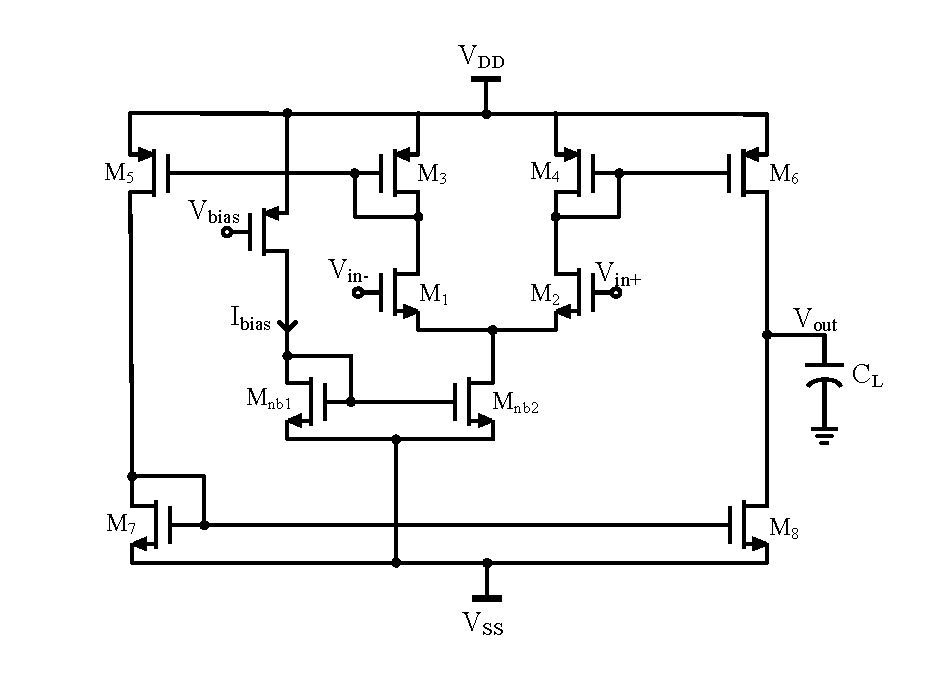
\includegraphics[scale=1]{Figures/Schematics/OTA_NMOS_Vbias.pdf}
\caption{Schematic of the OTA Designed}
\end{figure}

\begin{table} [H]
\centering
\begin{tabular}{@{}cccc@{}}
\toprule
Transistor			& Width				& Length			& Multiplier \\ \midrule
M1					& 6u				& 500n				&2			\\
M2					& 6u				& 500n				&2			\\ \bottomrule
\end{tabular}
\caption{Dimensions of the Transistors of the designed OTA}
\end{table}

\subsection{Test Setup}


\begin{figure} [H]
\centering
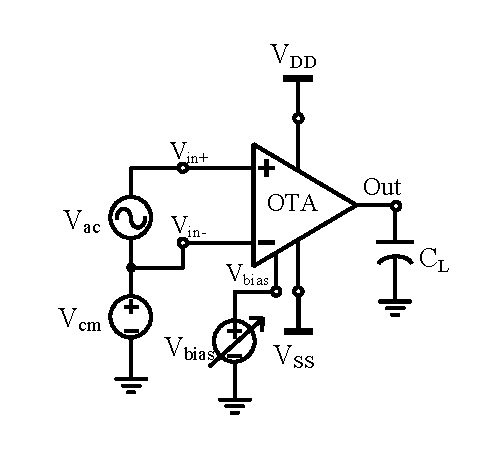
\includegraphics[scale=1]{Figures/Test_Benches/OTA/OTA_ACDC.pdf}
\caption{OTA Test setup for AC, DC and Noise Analysis}
\end{figure}


\begin{figure} [H]
\centering
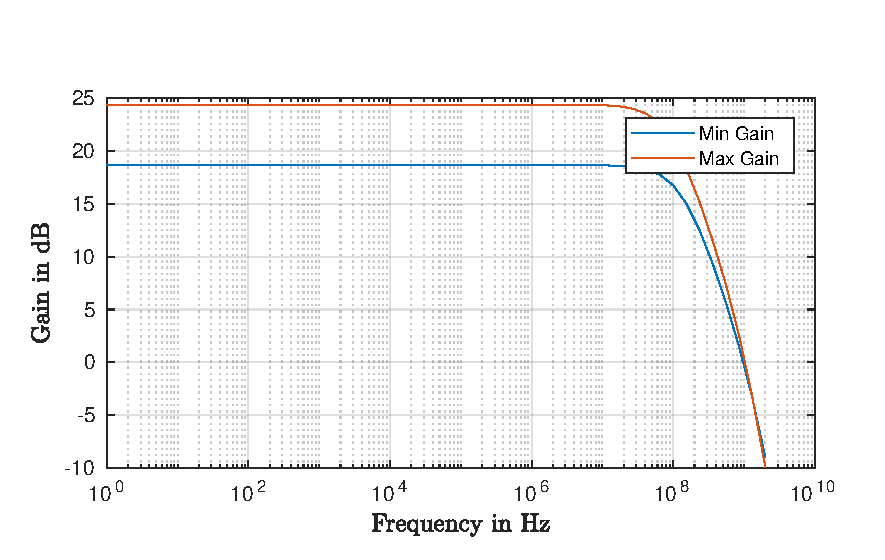
\includegraphics[scale=1]{Figures/Plots/OTA_Gain.pdf}
\caption{OTA Plot of Gain vs Frequency for different Vbias}
\end{figure}

\begin{figure} [H]
\centering
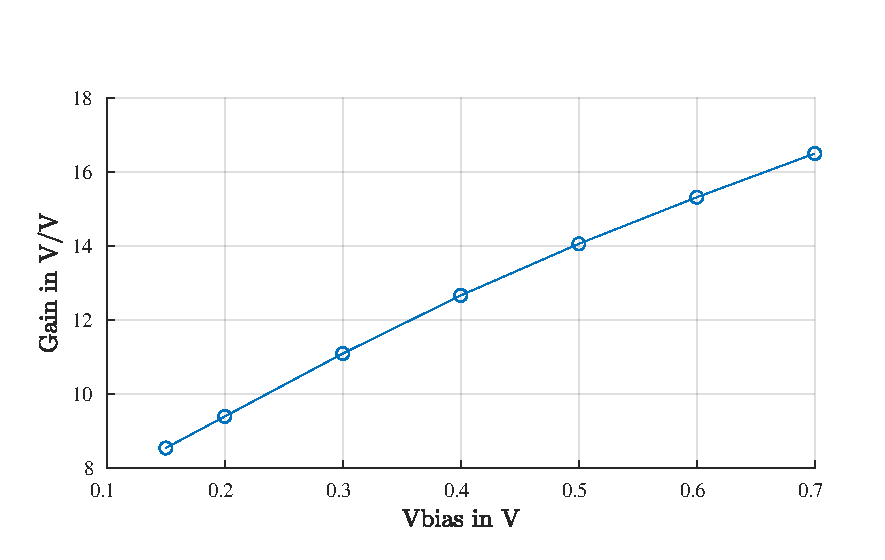
\includegraphics[scale=1]{Figures/Plots/OTA_Gain_Abs.pdf}
\caption{OTA Plot of Gain vs Vbias}
\end{figure}

\begin{figure} [H]
\centering
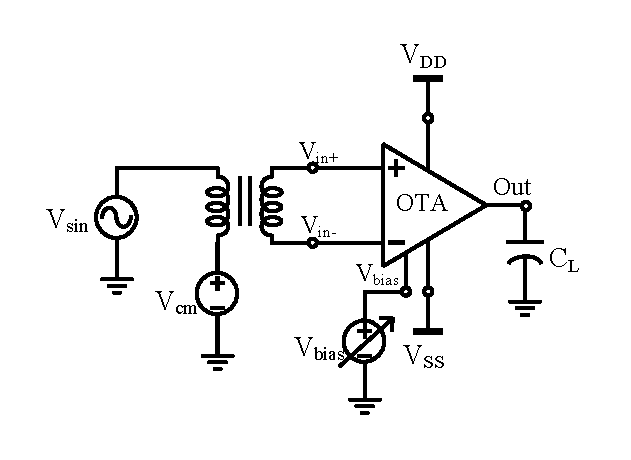
\includegraphics[scale=1]{Figures/Test_Benches/OTA/OTA_Sine.pdf}
\caption{OTA Test setup for Transient Analysis - Sine Wave Input}
\end{figure}

\begin{figure} [H]
\centering
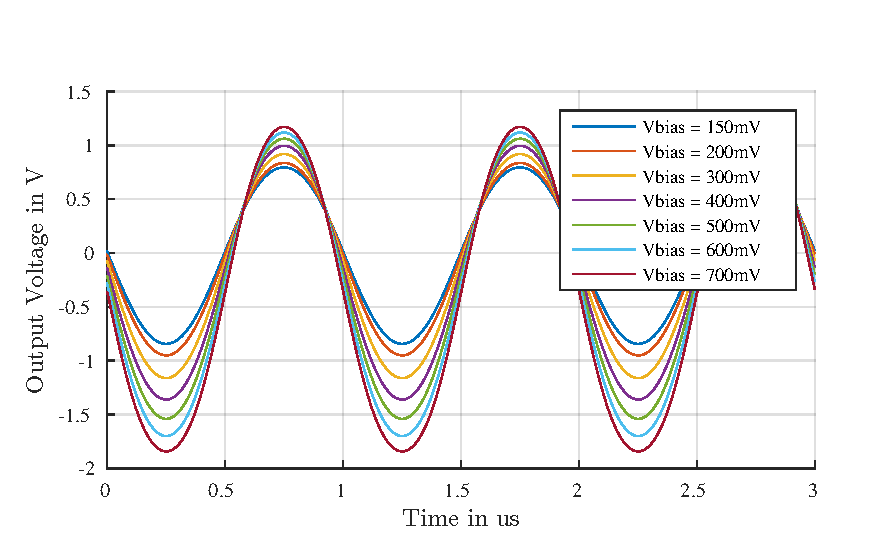
\includegraphics[scale=1]{Figures/Plots/OTA_Sine.pdf}
\caption{OTA Output Voltage for vs time for different Vbias}
\end{figure}

\begin{figure} [H]
\centering
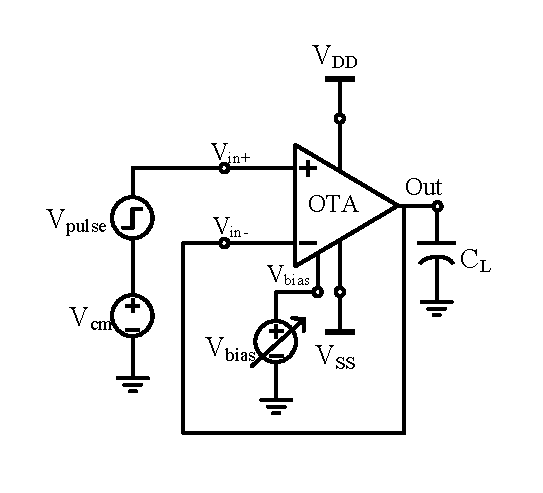
\includegraphics[scale=1]{Figures/Test_Benches/OTA/OTA_Slew.pdf}
\caption{OTA Test setup for Transient Analysis - Square Wave Input}
\end{figure}

\begin{figure} [H]
\centering
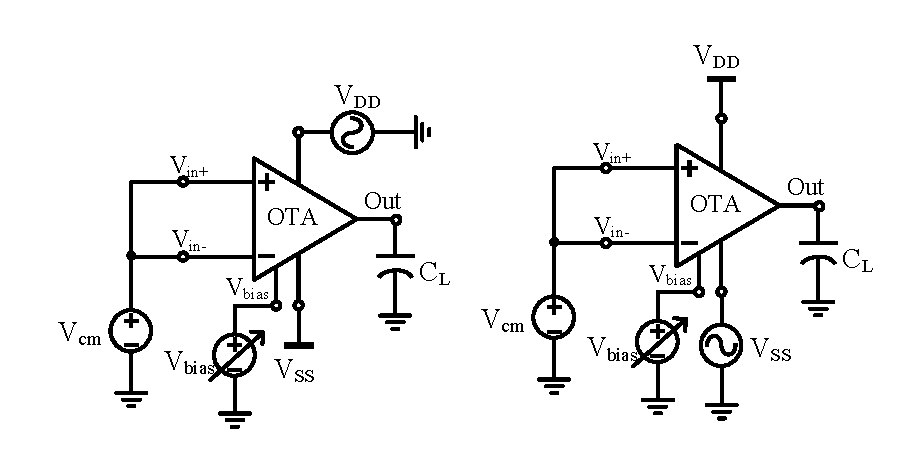
\includegraphics[scale=1]{Figures/Test_Benches/OTA/OTA_PSRR.pdf}
\caption{OTA Test setup for calculating PSRR}
\end{figure}

\begin{figure} [H]
\centering
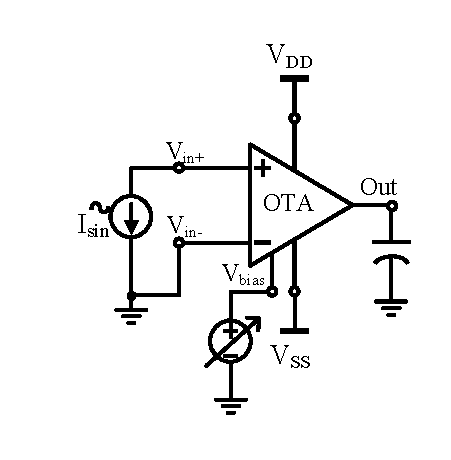
\includegraphics[scale=1]{Figures/Test_Benches/OTA/OTA_Zin.pdf}
\caption{OTA Test setup for calculating Input Impedance}
\end{figure}

\begin{figure} [H]
\centering
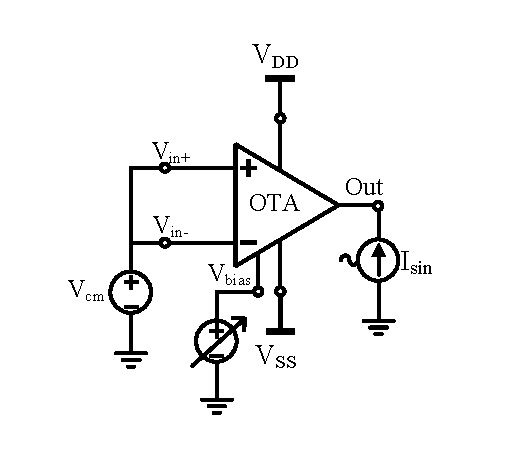
\includegraphics[scale=1]{Figures/Test_Benches/OTA/OTA_Zout.pdf}
\caption{OTA Test setup for calculating Output Impedance}
\end{figure}

\section{OP AMP Design}

\subsection{Schematic}
\begin{figure} [H]
\centering
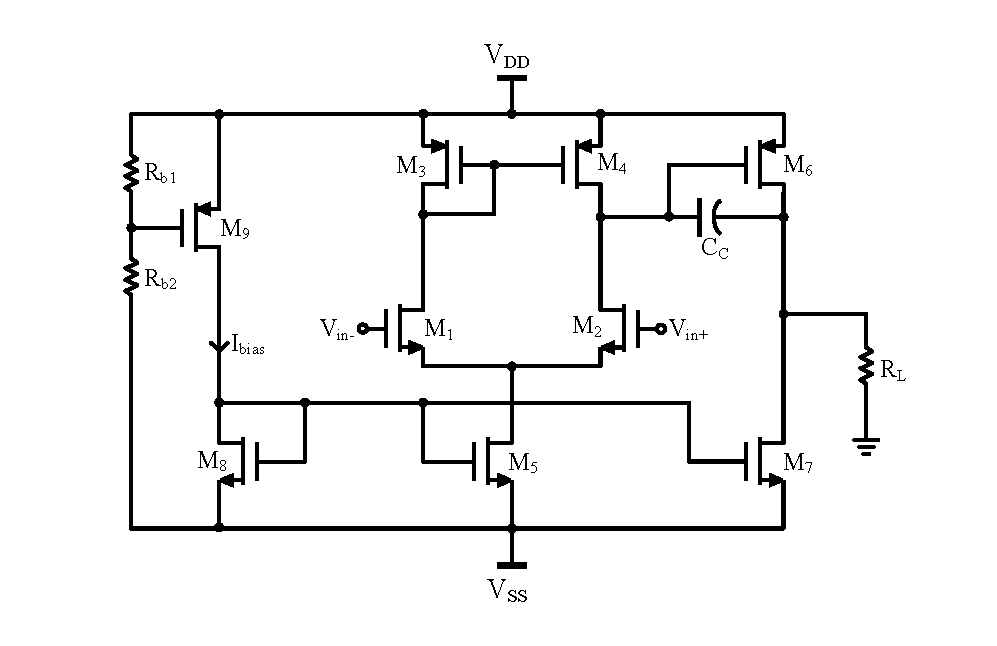
\includegraphics[scale=1]{Figures/Schematics/OPAMP_Vbias.pdf}
\caption{Schematic of the OPAMP Designed}
\end{figure}

\begin{table} [H]
\centering
\begin{tabular}{@{}cccc@{}}
\toprule
Transistor			& Width				& Length			& Multiplier \\ \midrule
M1					& 6u				& 500n				&2			\\
M2					& 6u				& 500n				&2			\\ \bottomrule
\end{tabular}
\caption{Dimensions of the Transistors of the designed OPAMP}
\end{table}

\subsection{Test Setup}

\begin{figure} [H]
\centering
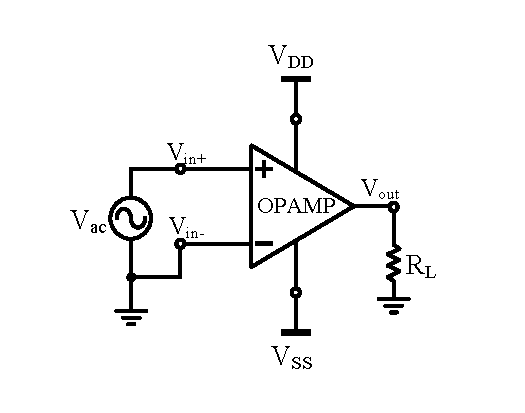
\includegraphics[scale=1]{Figures/Test_Benches/OPAMP/OPAMP_ACDC.pdf}
\caption{OPAMP Test setup for AC, DC and Noise Analysis}
\end{figure}

\begin{figure} [H]
\centering
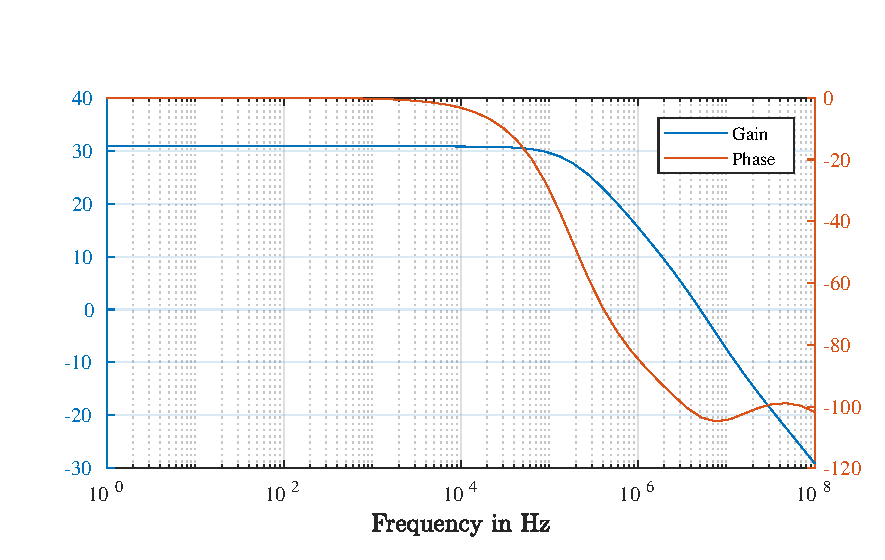
\includegraphics[scale=1]{Figures/Plots/OPAMP_Gain_PM.pdf}
\caption{OPAMP Plot of Gain and Phase vs Frequency}
\end{figure}

\begin{figure} [H]
\centering
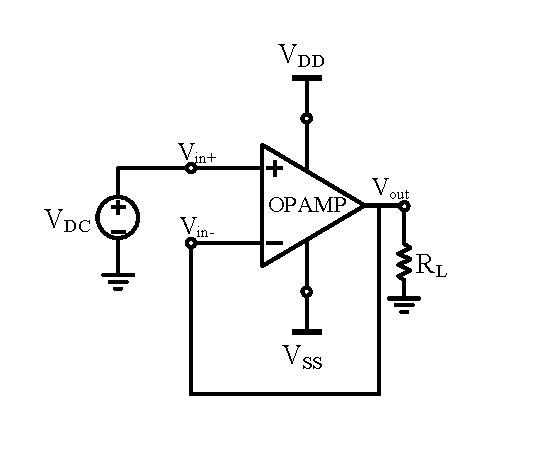
\includegraphics[scale=1]{Figures/Test_Benches/OPAMP/OPAMP_ICMR.pdf}
\caption{OPAMP Test setup for calculating ICMR}
\end{figure}

\begin{figure} [H]
\centering
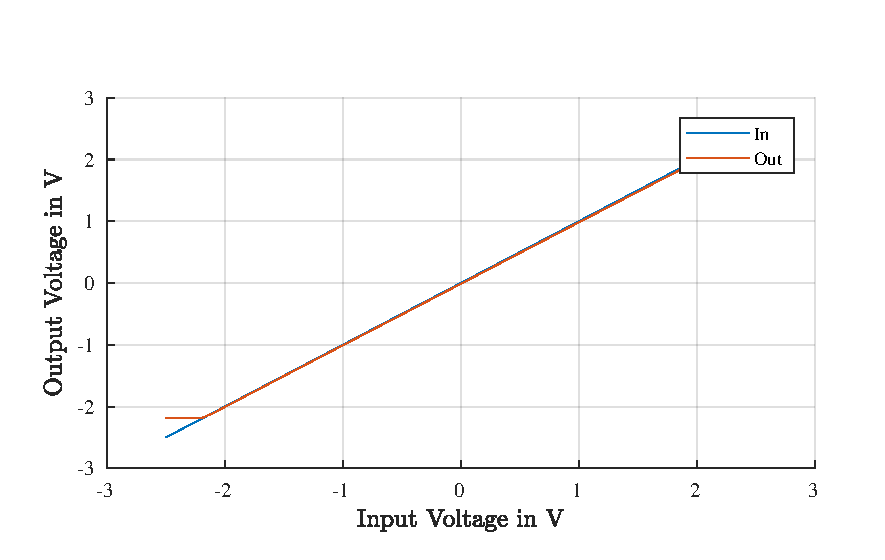
\includegraphics[scale=1]{Figures/Plots/OPAMP_ICMR.pdf}
\caption{OPAMP Plot of ICMR vs Vin}
\end{figure}

\begin{figure} [H]
\centering
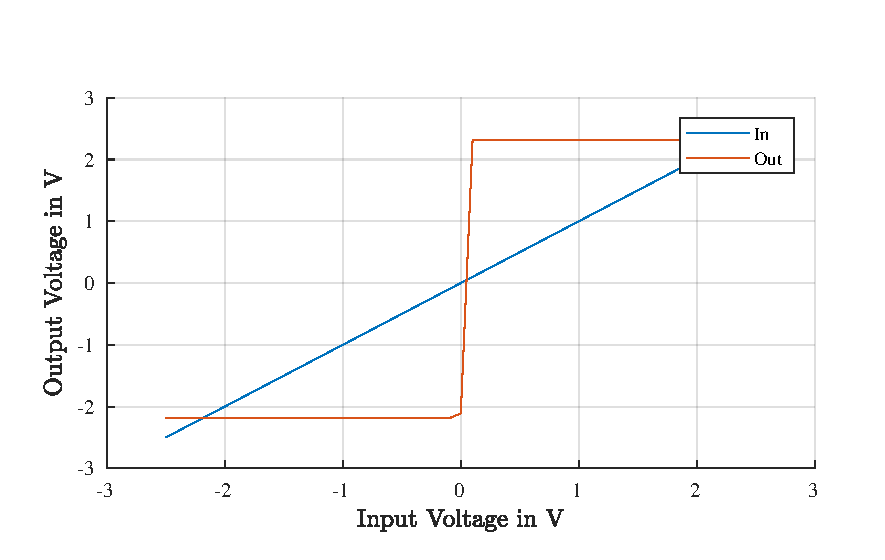
\includegraphics[scale=1]{Figures/Plots/OPAMP_OutSwing.pdf}
\caption{OPAMP Plot of Output Voltage Swing vs Vin}
\end{figure}

\begin{figure} [H]
\centering
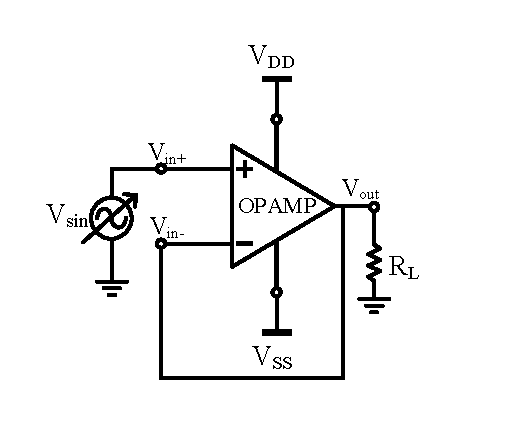
\includegraphics[scale=1]{Figures/Test_Benches/OPAMP/OPAMP_Sine.pdf}
\caption{Test setup for Transient Analysis - Sine Wave Input}
\end{figure}

\begin{figure} [H]
\centering
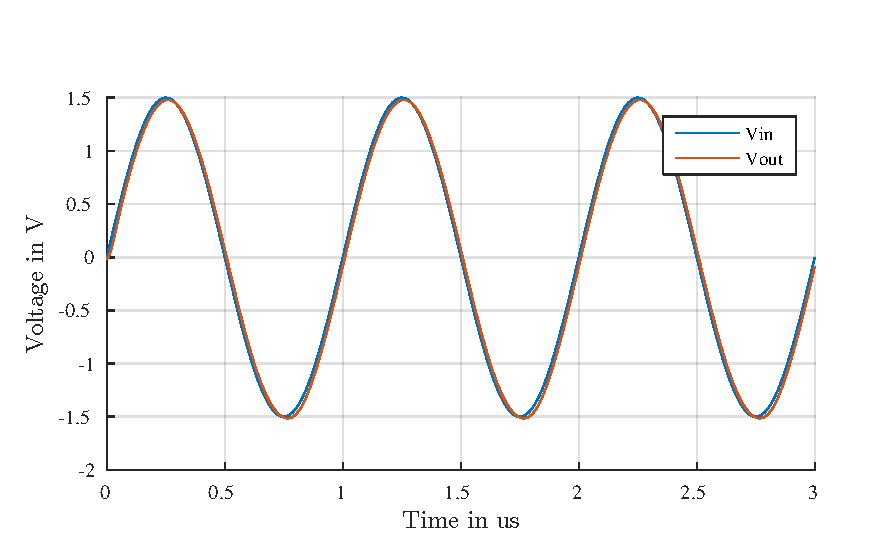
\includegraphics[scale=1]{Figures/Plots/OPAMP_Buffer.pdf}
\caption{OPAMP Plot of Output Voltage vs time}
\end{figure}

\begin{figure} [H]
\centering
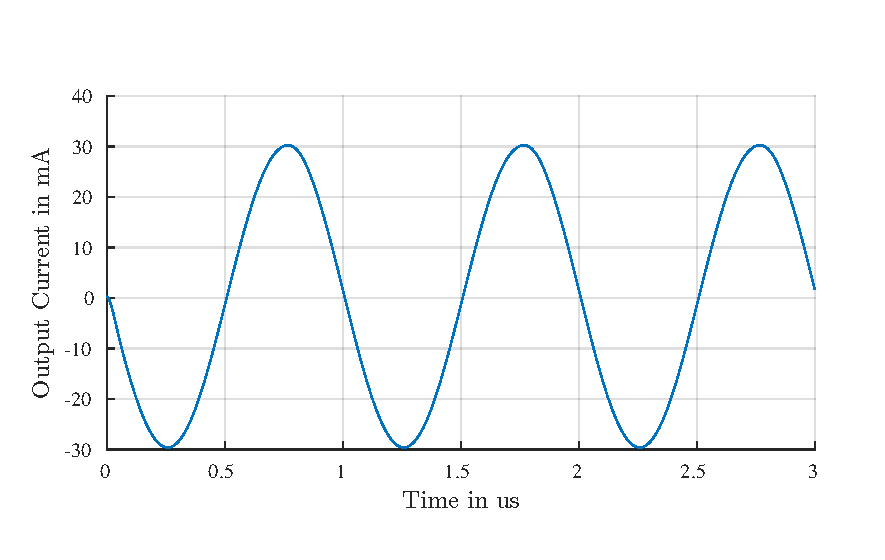
\includegraphics[scale=1]{Figures/Plots/OPAMP_Iout.pdf}
\caption{OPAMP Plot of Ourput Current vs time}
\end{figure}

\begin{figure} [H]
\centering
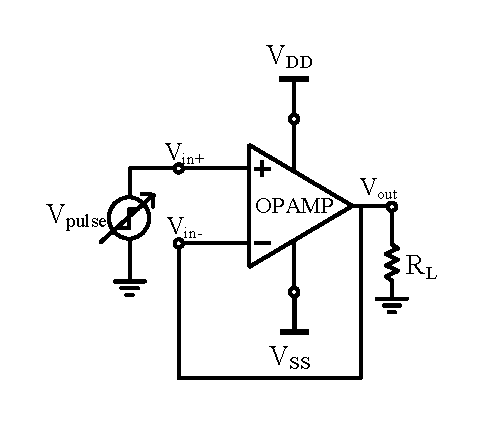
\includegraphics[scale=1]{Figures/Test_Benches/OPAMP/OPAMP_Slew.pdf}
\caption{Test setup for Transient Analysis - Square Wave Input}
\end{figure}

\begin{figure} [H]
\centering
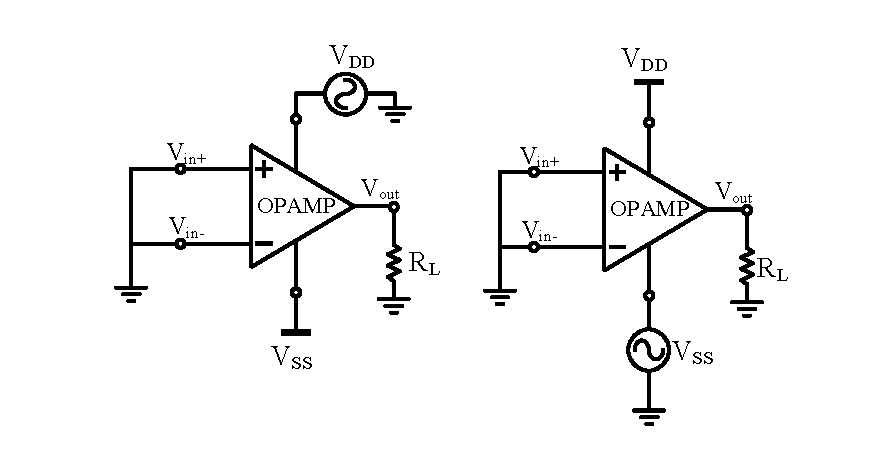
\includegraphics[scale=1]{Figures/Test_Benches/OPAMP/OPAMP_PSRR.pdf}
\caption{Test setup for calculating PSRR}
\end{figure}

\begin{figure} [H]
\centering
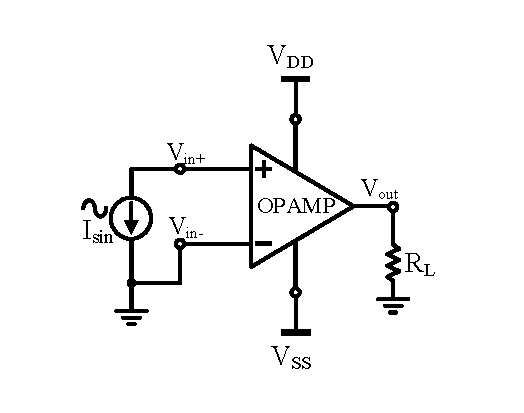
\includegraphics[scale=1]{Figures/Test_Benches/OPAMP/OPAMP_Zin.pdf}
\caption{Test setup for calculating Input Impedance}
\end{figure}

\begin{figure} [H]
\centering
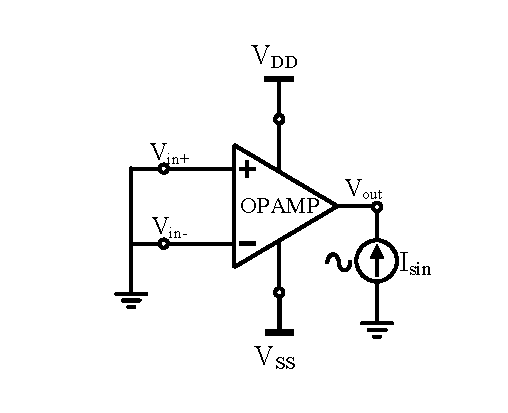
\includegraphics[scale=1]{Figures/Test_Benches/OPAMP/OPAMP_Zout.pdf}
\caption{Test setup for calculating Output Impedance}
\end{figure}

\section{The Complete Design}

\begin{figure} [H]
\centering
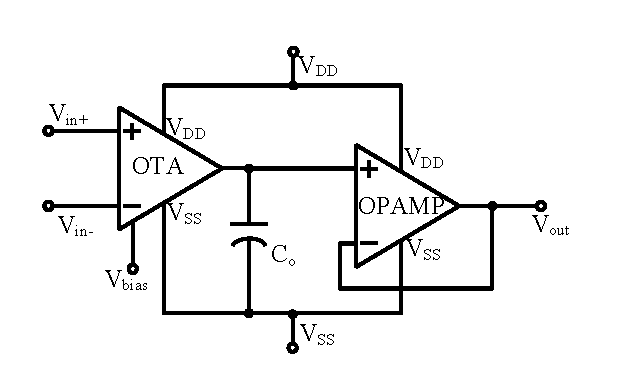
\includegraphics[scale=1]{Figures/System_Level/System_Overview.pdf}
\caption{Block Diagram of the Overall System}
\end{figure}

\begin{figure} [H]
\centering
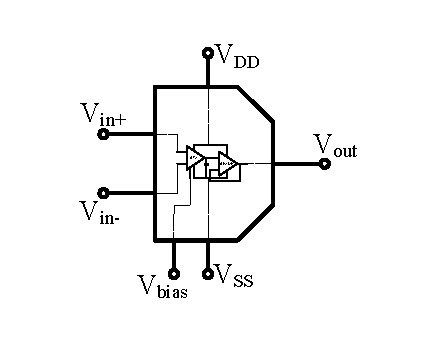
\includegraphics[scale=1]{Figures/System_Level/System_Symbol.pdf}
\caption{Schematic Symbol for the Overall System}
\end{figure}

\subsection{Schematic}

\begin{figure} [H]
\centering
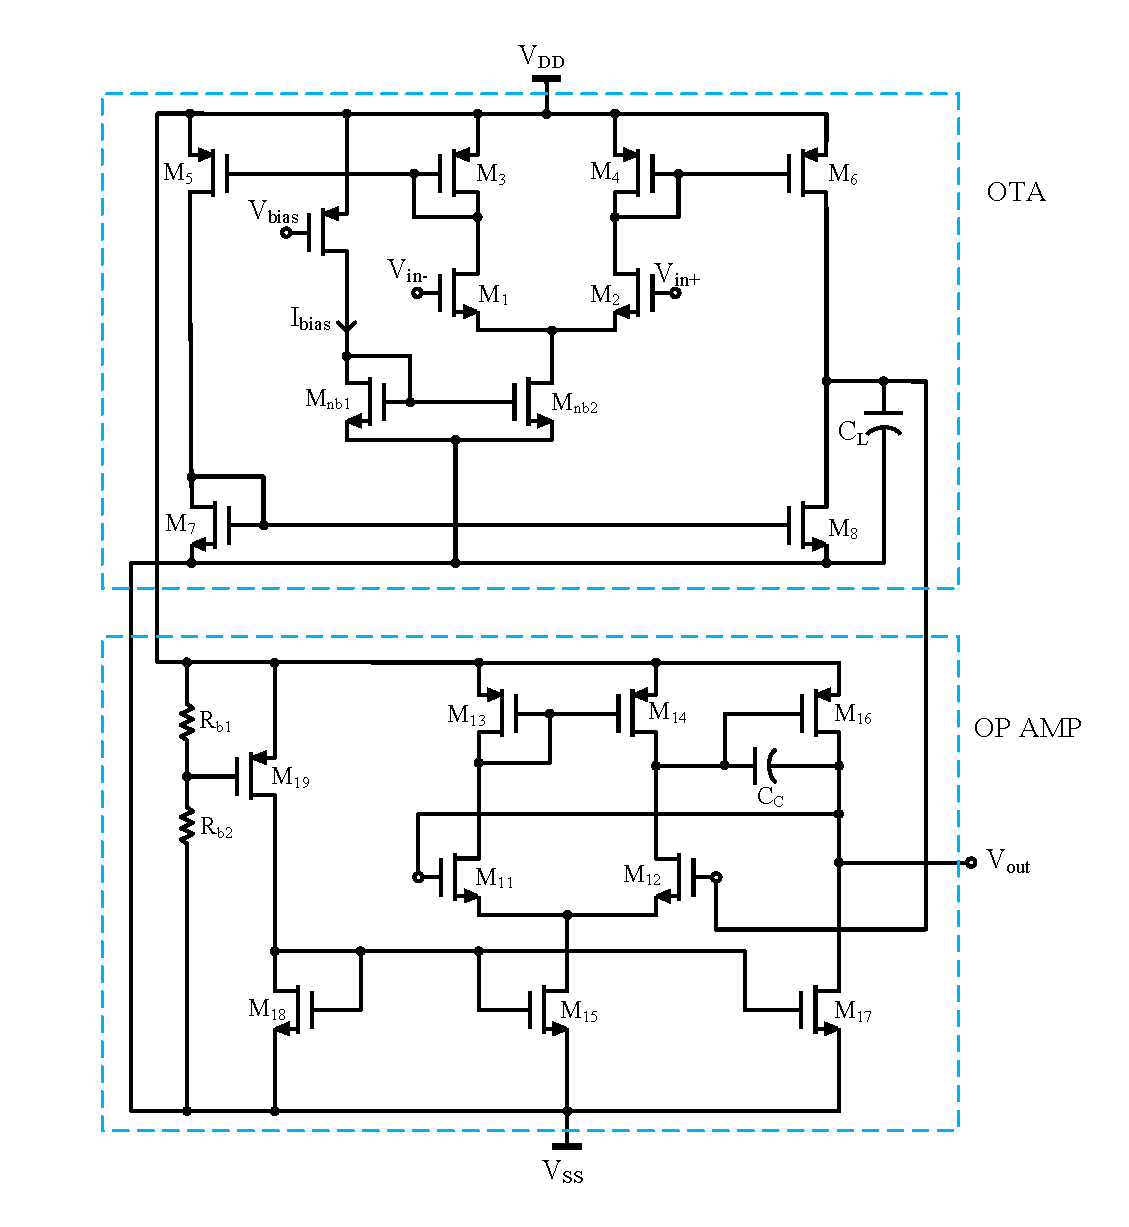
\includegraphics[scale=1]{Figures/Schematics/OTA_OPAMP_Schematic.pdf}
\caption{Schematic Diagram for the Overall System}
\end{figure}
